\chapter{Using Neural Networks to Detect Zebra Crosswalks}

\section{Input Image Constraints}
\label{Input Image Constraints}

Some image constraints were chosen for this scope of this paper because they would have been difficult to incorporate into this algorithm and were not necessary for a proof of concept implementation.

\begin{itemize}
\item All images are taken horizontally.
\end{itemize}

As detailed in future work, odd image angles can be very easily accounted for using the sensors of a phone, and the frame being horizontal makes image processing easier. Being able to assume that all true stripelets are horizontal removes them from the sample early on for being too vertical, or having a slope that is too far from the horizon. 

\begin{itemize}
\item All images contain crosswalks unaffected by shadows.
\end{itemize}

Shadows in a crosswalk create extremely strong lines that can interfere with the detection algorithm, as such they will be left for future work. 

\begin{itemize}
\item All crosswalks are white.
\end{itemize}

Yellow and white crosswalks have different pixel intensities, which may cause issues with the neural network training parameters, so in order to negate that issue, yellow crosswalks were excluded. 

\section{Algorithm Overview}
\label{Algorithm Overview}

\subsection{Stripelet Detection}

Following the method in the figure-ground paper \cite{Coughlan2006}, the frame is blurred slightly, and then converted to grayscale (Shown in figure \ref{fig:SlightlyBlurred}). 

\begin{figure}[t]
\begin{center}
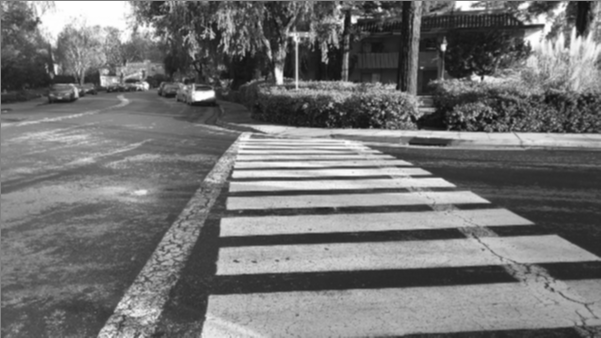
\includegraphics[width=7cm]{figures/SlightlyBlurredInput.png}
\captionfonts
\caption{Input image blurred and converted to grayscale}
\label{fig:SlightlyBlurred}
\end{center}
\end{figure}

The Sobel derivative is taken in the Y direction, leaving just the changes in the Y direction. The resulting pixels are either positive or negative, which signifies whether they are going from dark to light, or light to dark, giving us pixels that can be either the bottom or the top of the crosswalk. These are potential edges of crosswalks in the image (See figure \ref{fig:TopAndBottomSobel}). 

\begin{figure}[t]
\begin{center}
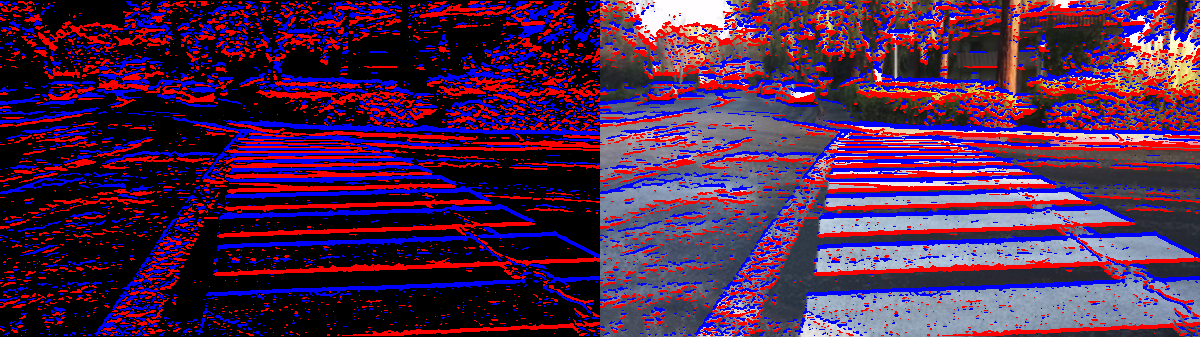
\includegraphics[width=14cm]{figures/TopAndBottomSobel.png}
\captionfonts
\caption{Sobel derivative of the image - positive values colored red, negative values colored blue}
\label{fig:TopAndBottomSobel}
\end{center}
\end{figure}

A standard method of Hough transform for line detection is then used to discover lines (figure \ref{fig:HoughLinesAfterMerge}). 

\begin{figure}[t]
\begin{center}
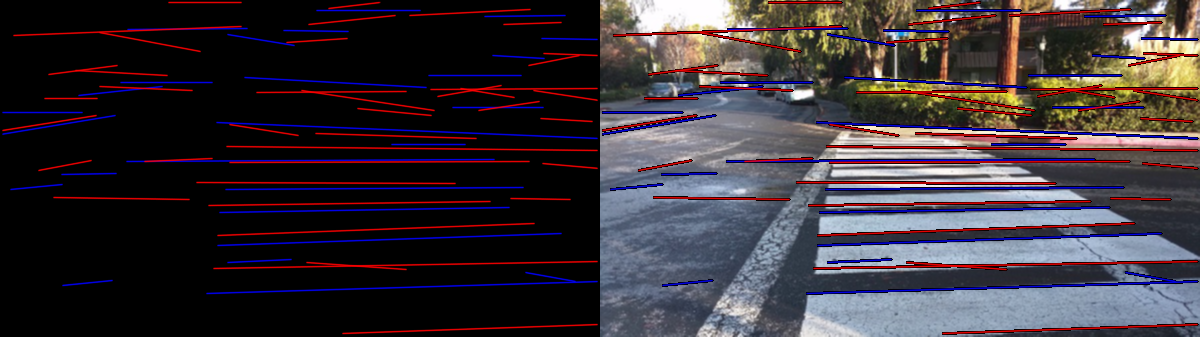
\includegraphics[width=14cm]{figures/HoughLinesAfterMerge.png}
\captionfonts
\caption{Lines detected using Hough transform on image from figure \ref{fig:TopAndBottomSobel} - blue is potential crosswalk top lines, red is potential  bottom lines}
\label{fig:HoughLinesAfterMerge}
\end{center}
\end{figure}

The generated lines are either defined as potential crosswalk top edges, or bottom edges. These potential edges are matched up against other edges (top vs bottom edges) to determine if they fit certain criteria to be considered stripelets. A stripelet is defined as an area bounded by a top and bottom line that follows certain constraints. The constraints used in Coughlan's figure-ground crosswalk paper \cite{Coughlan2006} are the same as used here: the top line is above the bottom line in the image, the two lines' slopes are very similar, the vertical width of the generated stripelet is between a defined cutoff value, and the two lines have sufficient X overlap. If all of these are true, then it is returned as a stripelet (See figure \ref{fig:UnculledStripelets}). 

\begin{figure}[t]
\begin{center}
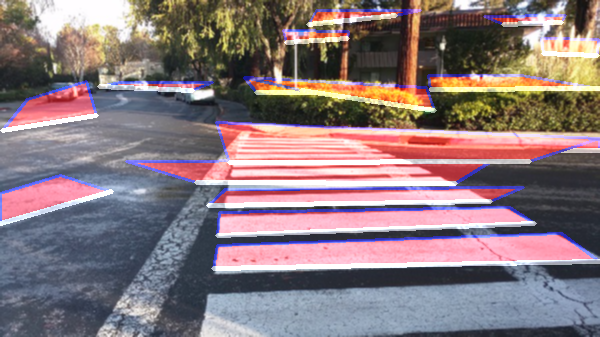
\includegraphics[width=7cm]{figures/UnculledStripelets.png}
\captionfonts
\caption{All of the stripelets detected after running the constraints on all the input lines from figure \ref{fig:HoughLinesAfterMerge}}
\label{fig:UnculledStripelets}
\end{center}
\end{figure}

\subsection{Neural Network Prediction of Crosswalk Stripelets}

%neural network based classification

At this point, the algorithm has generated a list of stripelets that are potentially part of a crosswalk. The inputs used for the neural network are a few parameters extracted from the image. The parameters are chosen because they possess characteristics that are believed may contribute towards helping identify a stripelet. A few sample parameters used are the stripelet's vertical/horizontal width, variance of the pixel intensity, and the lengths of the top and bottom lines. These numbers are calculated and then fed into the trained neural network, resulting in a very fast prediction as to whether or not that stripelet is part of a crosswalk.


Eleven different characteristics of the stripelets were chosen for use as the neural network parameters. The parameters are as follows:

\begin{enumerate}
   \item Bottom line length
   \begin{itemize}
     \item Description: The measure of the length of the bottom of the stripelet.
     \item Reasoning: Crosswalk stripelets are to have certain lengths, so this measure could help identify the validity of the stripelet.
   \end{itemize}
   \item Top line length
   \begin{itemize}
    \item Description: The measure of the length of the top of the stripelet.
    \item Reasoning: This value is similar to the bottom line length, and should pair well with the bottom length to give more information about the stripelet, as the two values are correlated.
   \end{itemize}
   \item Difference between top line length and bottom line length
   \begin{itemize}
     \item Description: The difference in length between the top and the bottom of the stripelet.
     \item Reasoning: Feeding in the difference between these measures explicitly could assist the neural network in using the difference. The bottom ought to be wider and the difference between the two should typically be a reasonably small number. 
   \end{itemize}
   \item Vertical stripelet width
   \begin{itemize}
     \item Description: The width of the stripelet vertically between the top and bottom lines.
     \item Reasoning: The vertical width of the stripelet is a useful factor because stripelets should have a certain vertical width that correlates with their top and bottom lengths, which would help define them as being part of a crosswalk.
   \end{itemize}
   \item Horizontal stripelet width
   \begin{itemize}
     \item Description: The width of the stripelet horizontally; the average length of the top and bottom lines.
     \item Reasoning: Similar to the vertical stripelet width, this parameter should correlate with the other parameters.
   \end{itemize}
   \item Vertical stripelet location
   \begin{itemize}
     \item Description: The vertical stripelet location (Y value of the stripelet center).
     \item Reasoning: The vertical stripelet location should help to correlate with other parameters to give a better prediction. For example, one might expect that a crosswalk stripelet higher in the image would be smaller, which would correlate this value with vertical and horizontal stripelet width. 
   \end{itemize}
   \item Variance of the stripelet pixel values
   \begin{itemize}
     \item Description: Pixel intensity variance within the stripelet.
     \item Reasoning: The pixel intensity variance should be lower for well painted stripelets, and high for stripelets that contain many different pixel values. This would be indicative of a non-crosswalk stripelet. 
   \end{itemize}
   \item Standard deviation of the stripelet pixel values
   \begin{itemize}
     \item Description: Square root of the variance.
     \item Reasoning: This measure may produce the same insights as the variance, and may allow a similar but simpler metric for the neural network to use.
   \end{itemize}
      \item Standard deviation of the pixel intensity of the area surrounding the stripelet
   \begin{itemize}
     \item Description: An area surrounding the stripelet is defined and the standard deviation of the pixel intensity in the area is found.
     \item Reasoning: The area around the stripelet should have a low standard deviation because it would be regular concrete without any lines for a crosswalk stripelet.
   \end{itemize}
      \item Standard deviation of the area surrounding the stripelet divided by standard deviation of the stripelet
   \begin{itemize}
     \item Description: The standard deviation of the area surrounding the stripelet divided by standard deviation of the stripelet.
     \item Reasoning: This ratio may help to give the neural network information about the relationship between the two measures.
   \end{itemize}
   \item Average stripelet pixel intensity divided by average pixel intensity of the area surrounding the stripelet
   \begin{itemize}
     \item Description: Average pixel intensity of the stripelet divided by the average pixel intensity of the area surrounding the stripelet.
     \item Reasoning: The stripelet pixel intensity should be much greater inside the stripelet than the area surrounding it, so this value could assist in finding which ratios are indicative of crosswalk stripelets or not. 
   \end{itemize}
\end{enumerate}

\subsection{Crosswalk Detection}

The stripelets that are predicted by the neural network to be part of a crosswalk are then checked one by one against the other stripelets through a manual feature comparison process. The compared features of the two stripelets are their average slopes, the horizontal pixel overlap, the vertical width of the stripelets, and the Y range overlap. The average slopes should be similar, the horizontal pixels should have a large amount of overlap, the vertical width of the stripelet which is lower in the image should be wider, as well as the horizontal width, and the Y ranges should have minimal overlap, if any. If two of the predicted crosswalk stripelets satisfy all of these constraints, then the image is declared to contain a zebra crosswalk. If all of the constraints fail to pass, then the image is not labeled a crosswalk. 

\subsection{Crosswalk Boundary Line Drawing}

In order to attempt to draw the boundary lines for the crosswalk, the edges from the stripelets that were positively identified as being part of a crosswalk are used. Three points are taken from the outer edges of the stripelets to assist in predicting the boundary as shown in figure \ref{fig:LinesAndEdgePoints}.  

\begin{figure}[t]
\begin{center}
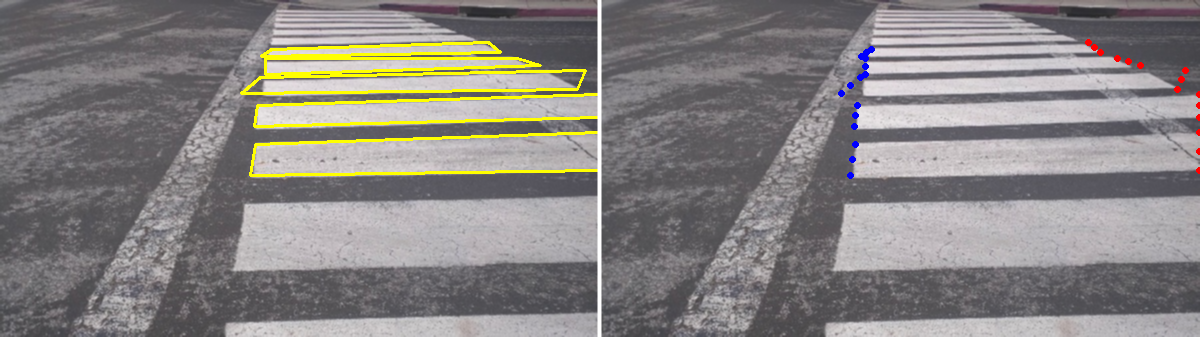
\includegraphics[width=14cm]{figures/LinesAndEdgePoints.png}
\captionfonts
\caption{Left to right: (a) Stripelets used to detect crosswalk. (b) Points taken from the edges of the stripelets}
\label{fig:LinesAndEdgePoints}
\end{center}
\end{figure}

RANSAC line fitting is applied to these points in order to fit a line that is the approximation of the edge line, shown in figure \ref{fig:LinesUsingJustGoodStartAndEnds}. 

\begin{figure}[t]
\begin{center}
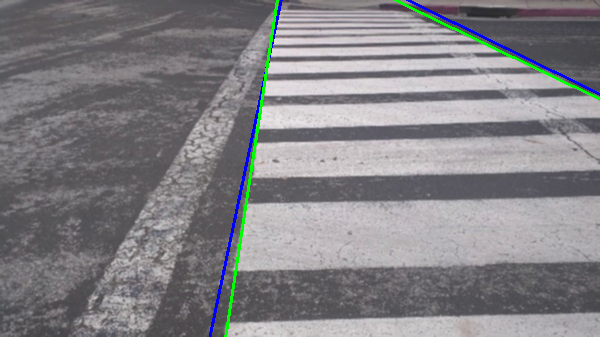
\includegraphics[width=7cm]{figures/LinesUsingJustGoodStartAndEnds.png}
\captionfonts
\caption{The green line is a manually drawn edge line, and the blue line is the estimated line}
\label{fig:LinesUsingJustGoodStartAndEnds}
\end{center}
\end{figure}